\documentclass[12pt, a4paper]{article}

\usepackage{tikz}
\usetikzlibrary{shapes.geometric}    % trapezium
\usetikzlibrary{arrows}              % arrow tips
\usepackage{amsmath, amsfonts}
\usepackage{bm}                      % boldsymbol
\usepackage{makecell}                % makecell
\usetikzlibrary{matrix,calc}
\usepackage{color}
\usepackage{xcolor}
\usepackage{multicol}
\definecolor{mygray}{HTML}{F0F0F0}
\definecolor{myred}{HTML}{CD594A} 
\definecolor{mygreen}{HTML}{829356} 
\definecolor{myblue}{HTML}{3C6478} 
\usepackage{mathtools}
\usetikzlibrary{decorations.pathreplacing}

\newcommand{\trans}{\text{T}}
\newcommand{\inv}{{-1}}
\newcommand{\eins}{\mathds{1}}
\DeclareMathOperator{\E}{\mathbb{E}}
\DeclareMathOperator{\I}{\mathbb{I}}
\newcommand{\tbf}[1]{\textbf{#1}}
\DeclareMathOperator{\tr}{tr}
\newcommand{\D}{\mathbf{D}}
\newcommand{\K}{\mathbf{K}}

\definecolor{mygray}{HTML}{F0F0F0}

\begin{document}


\begin{figure}[h!]
  \begin{minipage}{\linewidth}
    \centering
    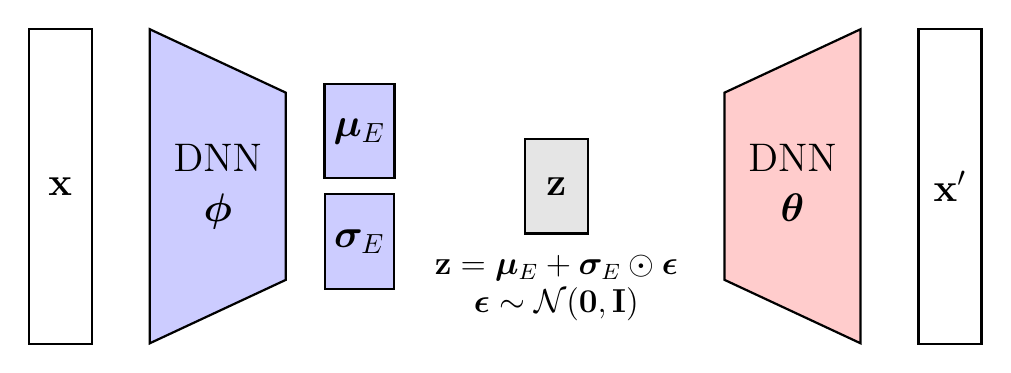
\begin{tikzpicture}[baseline=0, >=latex',thick, scale=1, every node/.style={scale=1}] 
      \node (rect) at (0,0)
      [draw, thick, minimum width=0.8cm, minimum height=4cm] {\Large{$\tbf{x}$}};

      \node [trapezium, trapezium angle=65, minimum width=4cm,
      inner xsep=0.3cm,
      draw, thick, rotate=-90, fill=blue!20] at (2,0)
      {\rotatebox{90}{\Large{\makecell[c]{DNN\\$\bm{\phi}$}}}};

      \node (rect) at (3.8,0.7)
      [draw, thick, minimum width=0.8cm, minimum height=1.2cm, name=mu, fill=blue!20]
      {\Large{$\bm{\mu}_E$}};

      \node (rect) at (3.8,-0.7)
      [draw, thick, minimum width=0.8cm, minimum height=1.2cm, name=sigma, fill=blue!20]
      {\Large{$\bm{\sigma}_E$}};

      \node (rect) at (6.3,0)
      [draw, thick, minimum width=0.8cm, minimum height=1.2cm, name=sigma, fill=gray!20,
      label={[yshift=-2.5cm]\large{\makecell[c]{$\tbf{z}=\bm{\mu}_E + \bm{\sigma}_E \odot \bm{\epsilon}$\\$\bm{\epsilon} \sim \mathcal{N} (\tbf{0}, \tbf{I})$}}}]
      {\Large{$\tbf{z}$}};
      
      \node [trapezium, trapezium angle=65, minimum width=4cm,
      inner xsep=0.3cm,
      draw, thick, rotate=90, fill=red!20] at (9.3,0)
      {\rotatebox{-90}{\Large{\makecell[c]{DNN\\$\bm{\theta}$}}}};
      
      \node (rect) at (11.3,0)
      [draw, thick, minimum width=0.8cm, minimum height=4cm] {\Large{$\tbf{x}^\prime$}};

    \end{tikzpicture}
  \end{minipage}
\end{figure}

\end{document}
